\documentclass{article}
\usepackage{fullpage,graphicx}
\usepackage{hyperref}
\usepackage[
  backend=bibtex,
  style=numeric,
  maxcitenames=2]{biblatex}
\addbibresource{ref}

\usepackage[dvipsnames,svgnames,x11names]{xcolor}
\usepackage{textcomp,listings,lstparams,lstcoq}
\lstdefinestyle{customcoq}{
  language=Coq,
  literate={<>}{$\ne$}1
  {->}{$\to$}1
}
\lstdefinestyle{json}{
  language=Coq
}
\newcommand{\ilc}[1]{\lstinline[style=customcoq]{#1}}

\usepackage{draft} % local
\newif\ifdraft\drafttrue
\newnote{lys}{BrickRed}
\newnote{bcp}{Chocolate}
\newnote{sz}{violet}

\title{From Interaction Trees to Asynchronous Tests}
\author{Yishuai Li}
\begin{document}
\maketitle
\section{Introduction}
Importance of rigorous testing in software development.

Main challenge: nondeterminism in various parts of the system.

Goal: a systematic testing framework for networked systems, addressing internal
nondeterminism and network nondeterminism.

Methodology: interpret model specification into testing logic; introduce
abstract representation for test input generation and shrinking.

Broader impact: Handling network nondeterminism is the first step towards
testing generic concurrent systems.  Automatically deriving tests from formal
specifications enables iterative incremental development of reliable software.

Todo thesis claim.  What technology solves what problem.

5--6 pages.

\section{Background}
Property-based testing with QuickChick.  Limitation: nondeterminism makes
validation logic hard to write.

ISSTA related work.

5--6+ pages.

\section{Prior Results}
Model-based testing in ISSTA paper.

Refactor previous paper.

\section{Research Plan}
\subsection{Test Input Generation and Shrinking}

One challenge for random testing is that, to find failing examples efficiently,
it is important to generate fairly large test cases.  But then, after a failing
test case has been found, it is important to \textit{minimize} the test input to
eliminate the parts that are not relevant to provoking the failure.  Tools like
QuickCheck therefore provide automatic methods for minimizing, or {\em
  shrinking}, failing tests, by incrementally generating smaller variants until
they reach a local minimum---a counterexample that cannot be reduced any
further.

Traditional shrinking doesn't work well for impure programs, which might mutate
state or interact with their environments, because an interesting test input in
one execution might become trivial or irrelevant in another run.  In particular,
when testing an interactive program, interesting test inputs might depend on
existing observations of the program's behavior.

To generate and shrink inputs that are interesting among different executions,
\textcite{Hughes2007} introduced a method that relates inputs to runtime
observations.  In this framework, the tester interacts with the system under
test (SUT) via function calls, and maintains a runtime state that is updated
after each call returns.  Test inputs are represented in an abstract language
that depends on the runtime state {\it e.g.} ``call function \ilc{foo(x)}, where
\ilc{x} is the return value of the 10th function call''.  Such abstract
representation is instantiated into a concrete input during runtime, by
remembering the 10th call's return value \ilc{a} to build the actual function
call \ilc{foo(a)}.

This methodology has achieved good results in testing state
machines~\cite{Hughes2016}, but the specification language requires the
interactions to be synchronous {\it i.e.} to return immediately upon call.
However, when testing networked systems, requests and responses might be delayed
or reordered \textit{en route}.  Such a scenario requires a different
specification language that allows asynchronous
interactions~\cite{li2021modelbased}, introducing new challenges in minimizing
test inputs, {\it e.g.} when a dependent response has not arrived.

I'll propose a generic method for generating and minimizing asynchronous test
interactions, by combining the idea of abstract input representation
from~\textcite{Hughes2007} with the asynchronous specification language
of~\textcite{li2021modelbased}.  The tester records a {\em trace} of network
packets sent and received, and uses the trace to instantiate abstract inputs
into concrete requests to send.  The key inovation is an intermediate
representation (IR) between structured application messages and bytes.  The IR
allows the generated abstract input to refer to specific fields in the trace,
and can handle situations where the referred field is absent (caused by internal
or network nondeterminism).

\subsubsection{Overview}
\begin{figure}
  \centering
  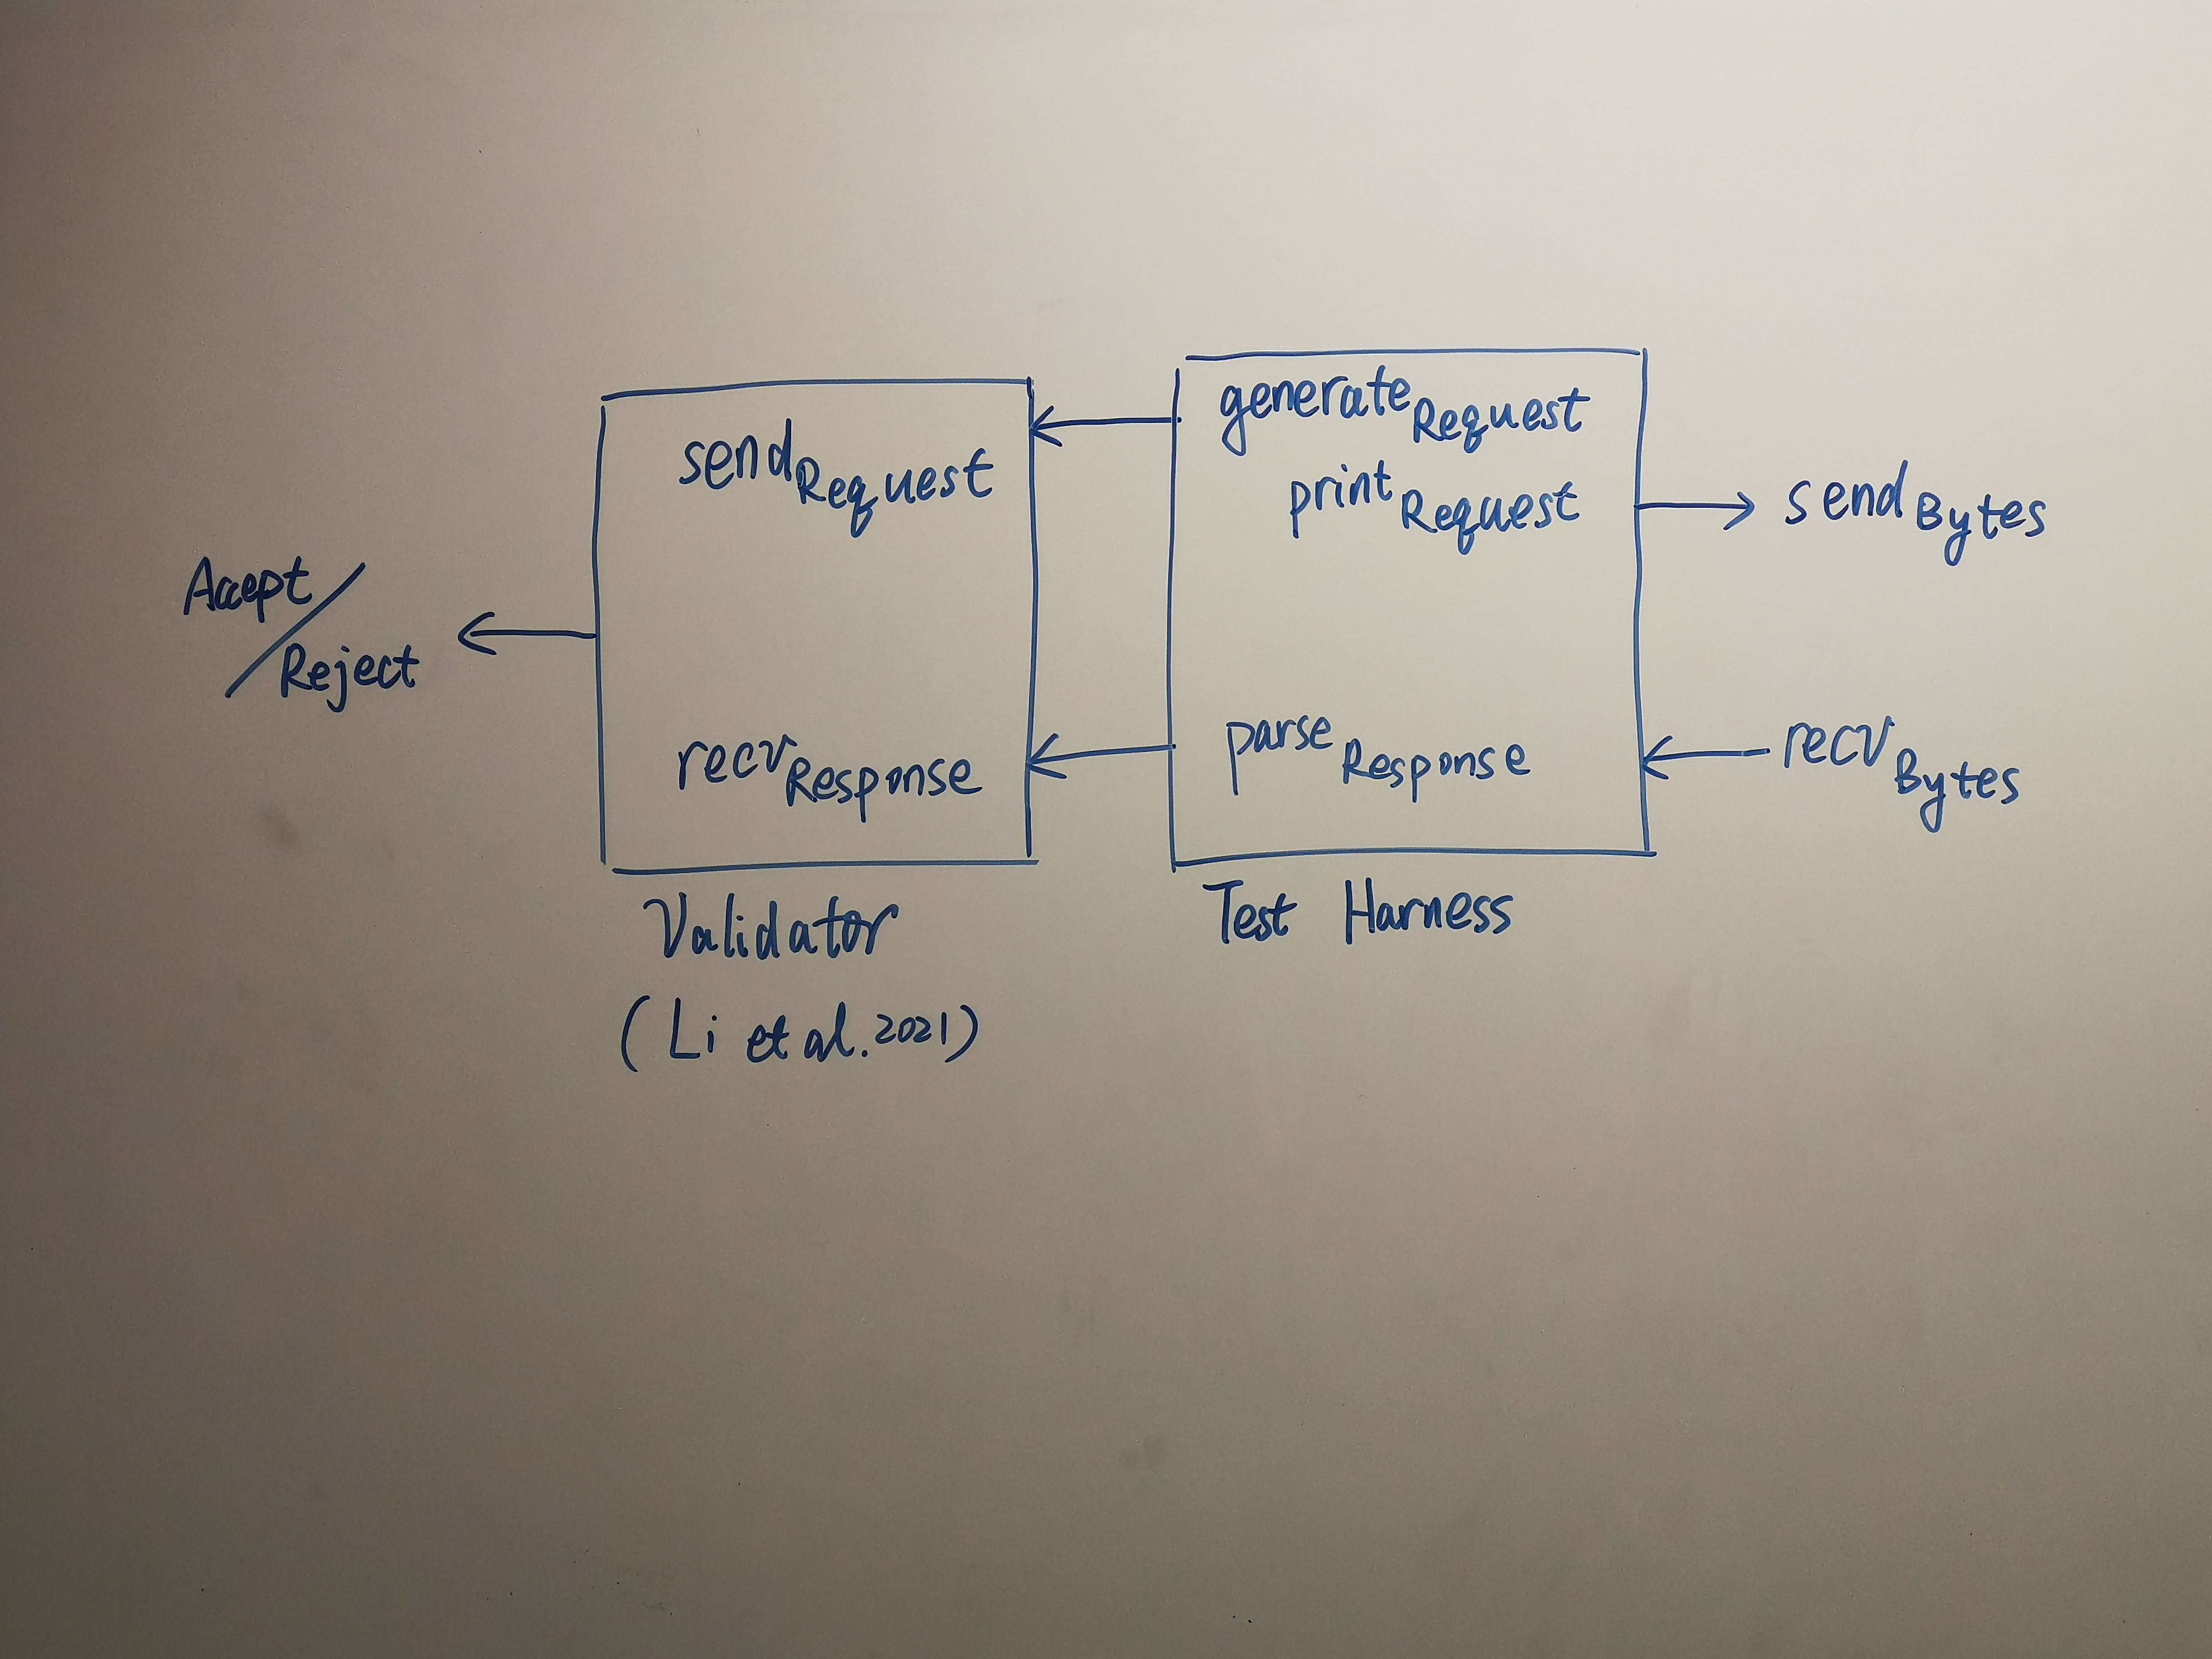
\includegraphics[width=.9\textwidth]{figures/overview}
  \caption{Test framework overview}
  \label{fig:overview}
\end{figure}

As shown in \autoref{fig:overview}, the test framework consists of a {\em
  validator} that determines whether the SUT's behavior satisfies the
specification, and a {\em test harness} that provides test inputs for the
validator.

A {\em validator} is a client-side model program that observes messages sent and
received and decides whether these interactions are conformant to the
specification.  For example, a simple validator for echo server is written as:
\begin{lstlisting}[style=customcoq]
  let validateEcho =
    request := sendRequest();
    response := recvResponse();
    if response <> request
    then reject
    else validate
\end{lstlisting}
Notice that the \ilc{sendRequest} event does not take the request to be sent as
argument, but in stead returns the request actually sent.  The validator only
describes the logic that checks messages sent and received, while the test
harness computes what requests to send.

The {\em test harness} takes a validator and turns it into an executable program
that performs network interactions.  It handles the validator's send and receive
events, and generates the requests to be sent.  A simple test harness for the
validator above is written as:
\begin{lstlisting}[style=customcoq]
  let execute(v) =
    match v with
    | x := sendRequest(); v'(x) =>
      request := arbitraryRequest();
      sendBytes(print(request));
      execute(v'(request))
    | x := recvRequest(); v'(x) =>
      responseBytes := recvBytes();
      execute(v'(parse(responseBytes)))
    | reject => reject
    end in
  execute(validateEcho)
  (* ... is equivalent to ... *)
  let executeValidateEcho =
    request := arbitraryRequest();
    sendBytes(print(request));
    responseBytes := recvBytes();
    if parse(responseBytes) <> request
    then reject
    else executeValidateEcho
\end{lstlisting}

The \ilc{arbitraryRequest} generator here produces requests randomly.  To
generate requests that depend on previously observed messages, my framework will
extend the test harness in \autoref{fig:overview} that records a trace of
messages.

\subsubsection{Architecture}
\begin{figure}
  \centering
  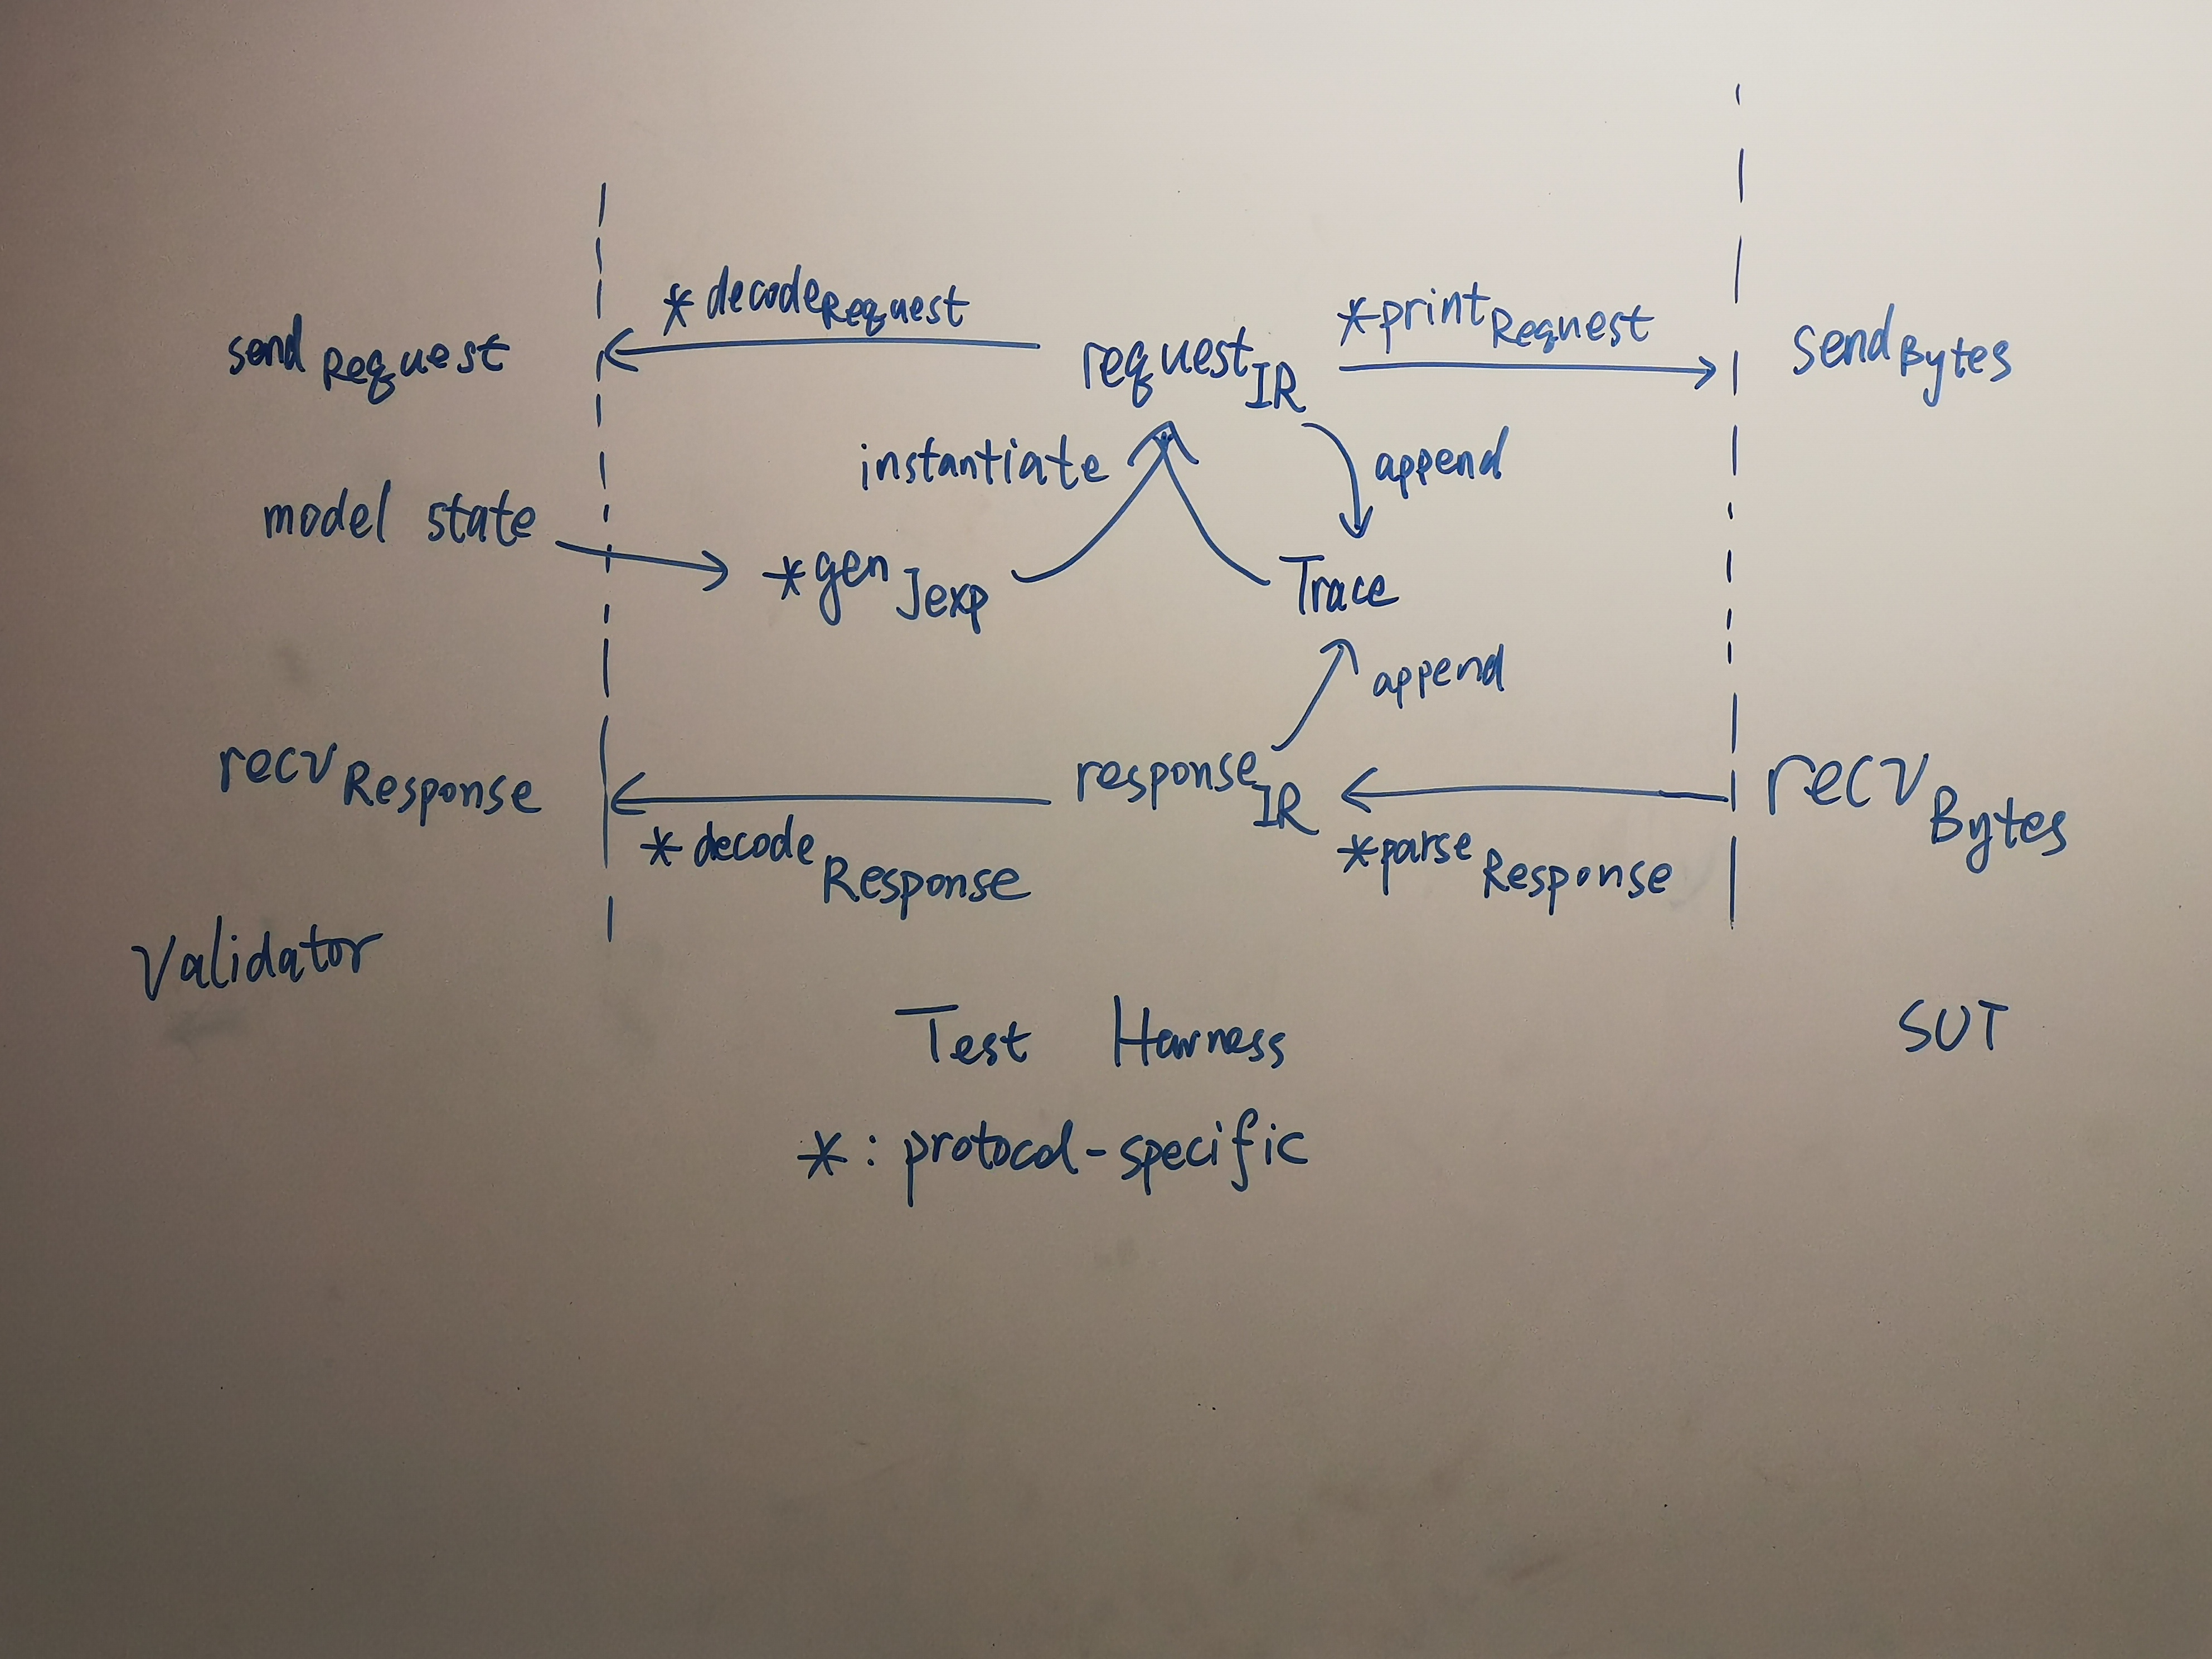
\includegraphics[width=.9\textwidth]{figures/harness}
  \caption{Test harness mechanism}
  \label{fig:harness}
\end{figure}

As shown in \autoref{fig:harness}, the test harness records a trace of requests
and responses, using an generic intermediate representation.  Requests are
generated as ``J-expressions'' that can be instantiated into a request IR based
on the trace.  For each protocol to test, the developers need to specify how to
generate J-expressions that represent requests.  Developers also need to define
how to interpret among the IR, bytes, and application messages.

\subsubsection{Intermediate representation language}
The purpose of introducing an IR in this framework is to enable a generic method
for generating requests that refer to specific fields in the trace.  For
example, when testing conditional HTTP requests, the generator wants to include
``a precondition that uses the ETag field of a previous response''; when testing
an online store, the generator wants to provide ``an order ID that the server
has mentioned before''.

I choose JSON as the intermediate representation.  Since JSON itself is widely
used in web applications, the IR should provide the flexibility for developers
to refer to any field in a JSON message, which might involve arbitrarily deep
path down the syntax tree.  \autoref{fig:ir} shows the intermediate
representation for two protocols.

\begin{figure}
  \begin{lstlisting}[style=customcoq]
    Example response1 : http_response :=
      Response (Status (Version 1 1) 200 (Some "OK"))
               [Field "ETag" "tag-foo";
                Field "Content-Length" "11"]
               (Some "content-bar").

    Example response2 : store_response :=
      Response__ListOrders [(233, (12, 100, 34, 500));
                            (996, (56, 400, 78, 20))].
  \end{lstlisting}
  \begin{minipage}[t]{.4\textwidth}
    \begin{lstlisting}[style=json]
      {
        "version": {
          "major": 1,
          "minor": 1
        },
        "code": 200,
        "reason": "OK",
        "fields": {
          "ETag": "tag-foo",
          "Content-Length": "11"
        },
        "body": "content-bar"
      }
    \end{lstlisting}
  \end{minipage}%
  \begin{minipage}[t]{.4\textwidth}
    \begin{lstlisting}[style=json]
      {
        "code": 200,
        "orders": [
          {
            "ID": 233,
            "BuyerID": 12,
            "BuyAmount": 100,
            "SellerID": 34,
            "SellAmount": 500
          },
          {
            "ID": 996,
            "BuyerID": 56,
            "BuyAmount": 400,
            "SellerID": 78,
            "SellAmount": 20
          }
        ]
      }
    \end{lstlisting}
  \end{minipage}
  \caption{Application message example for HTTP and online store protocols, and
    their corresponding intermediate representation}
  \label{fig:ir}
\end{figure}

To represent the correspondence between requests and responses, the trace labels
each message, and the request-response pair have the same label.
\autoref{fig:trace} shows a trace of messages sent and received by the tester
client.

\begin{figure}
  \begin{minipage}{.5\textwidth}
    \begin{lstlisting}[style=json]
      [
        {
          "label": 10,
          "message": {
            "method": "GET",
            "path": "index.html"
          }
        },
        {
          "label": 20,
          "message": {
            "method": "DELETE",
            "path": "index.html"
          }
        },
        {
          "label": 20,
          "message": {
            "code": 204,
            "reason": "No Content",
          }
        },
        {
          "label": 10,
          "message": {
            "code": 410,
            "reason": "Gone"
          }
        }
      ]
    \end{lstlisting}
  \end{minipage}%
  \begin{minipage}{.5\textwidth}
    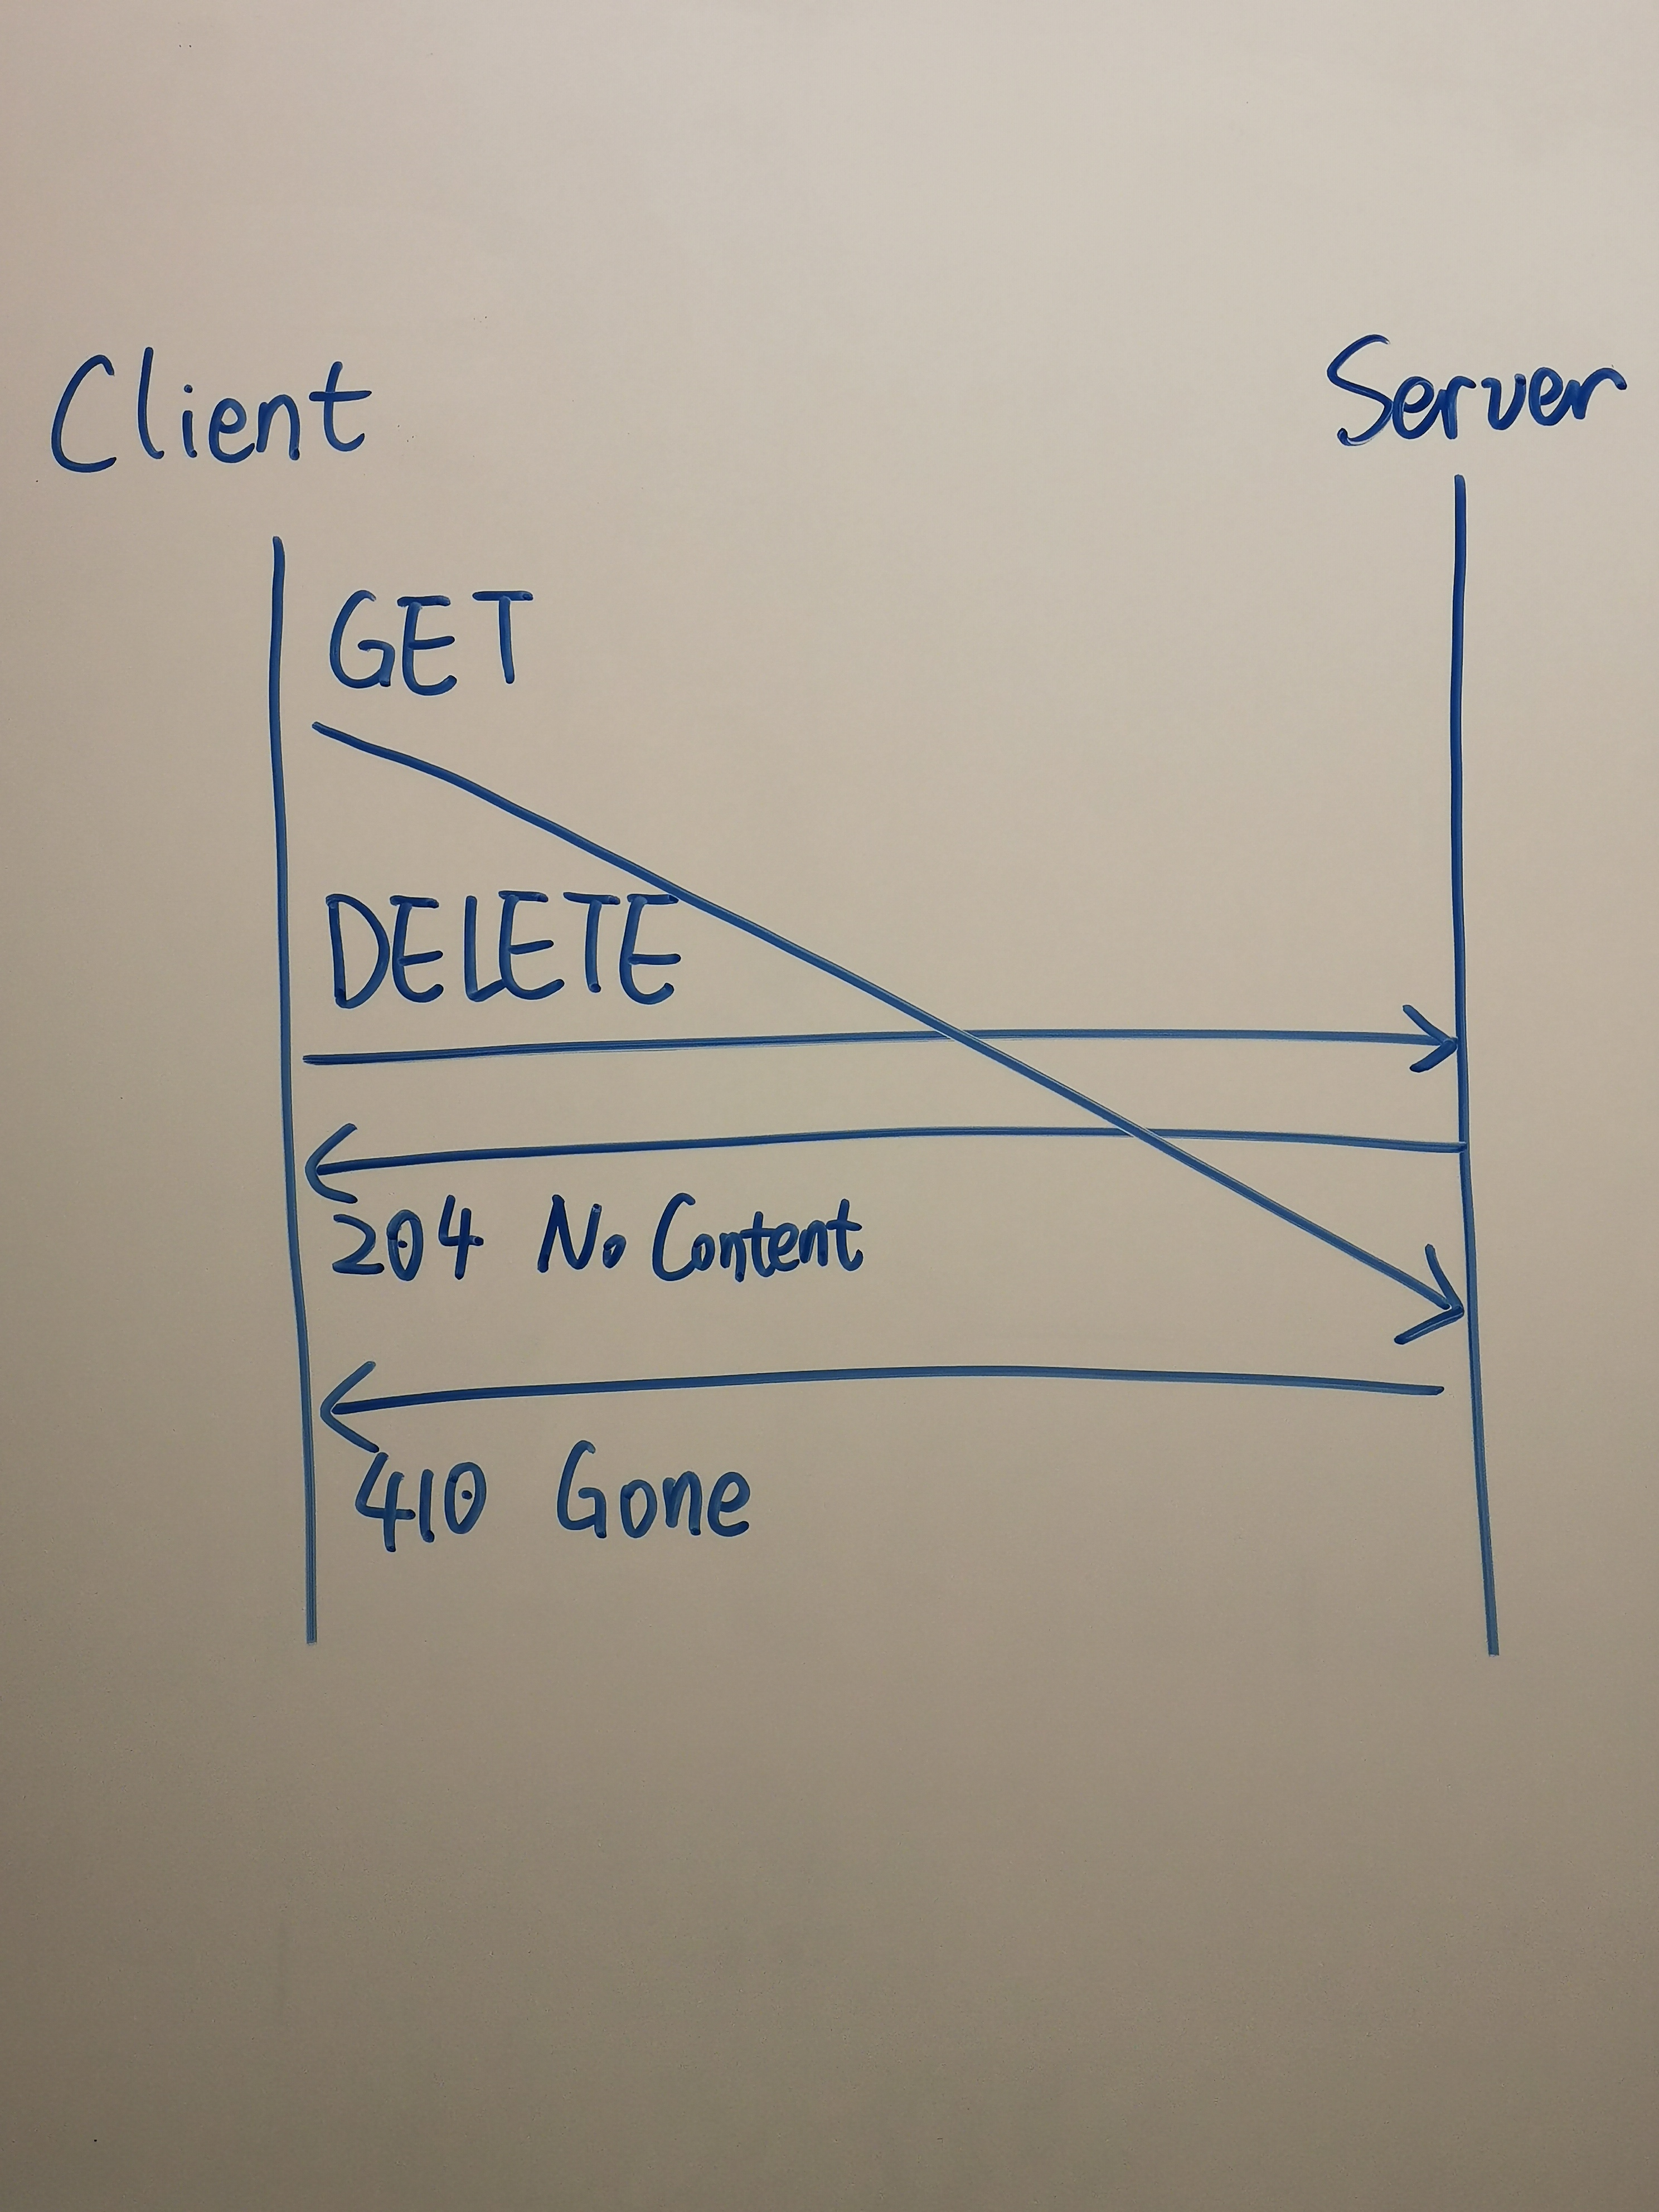
\includegraphics[width=\textwidth]{figures/trace}
  \end{minipage}
  \caption{Example client-side trace and its corresponding IR}
  \label{fig:trace}
\end{figure}

Based on this unified structure of messages, I introduce a symbolic language for
representing requests, called ``J-expressions''.  The J-expression is similar to
JSON, except that it allows a pointer notation that refers to the trace.  For
example, the following J-expression represents a \ilc{takeOrder} request whose
order ID is equal to the second order's ID in the message labelled 30:

\begin{lstlisting}[style=customcoq]
  Example xreq2 : jexp :=
    object [
      ("method", "takeOrder"); ("user", 2);
      ("order", ref 30 (this@"orders"#2@"ID") id)].
\end{lstlisting}

Notice the \ilc{ref} in the final line: The first argument 30 is the message
label in the trace.  The following \ilc{this@"orders"#2@"ID"} is a path for the
generator to search in the IR, pronounced ``the `ID' field in the 2nd entry of
the array named `orders' ''.  The last argument is the transformer function that
maps the found field to the generated request, here \ilc{id} means the found
order ID is used in the result request verbatim.

Suppose a trace contains a message labelled 30, and its payload is the second
example in \autoref{fig:ir}, then the request generator can find the
corresponding order ID in the request {\it i.e.}  996, and construct the
following request IR based on the J-expression above:

\begin{lstlisting}[style=json]
  {
    "method": "takeOrder",
    "user": 2,
    "order": 996
  }
\end{lstlisting}

\subsection{Generic specification language}
Based on my experiments on various web applications, I'll propose a generic
library for specifying application-level protocols.  Developers use the
domain-specific language to define protocol-specific aspects {\it e.g.}
prototype logic, message encoding {\it etc.}  and the library automatically
derives the specification into an interactive tester client that can reveal
servers' incomformance effectively.

5--6+ pages.  Include technical details for evaluation.

Timeline towards dissertation.  Month-level schedule, including publication.

\printbibliography

\end{document}
